\chapter{Onde piane TE e TM tra due materiali} 
\begin{figure}[h]
    \centering
    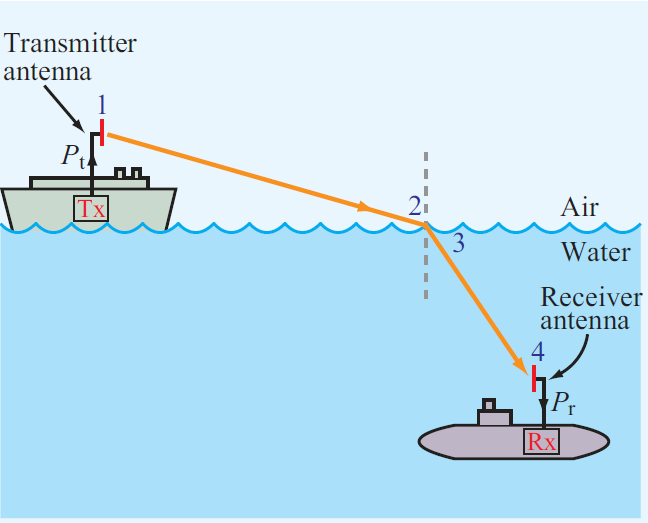
\includegraphics{TX and RX.PNG}
    
\end{figure}    

\newpage 

\section{Riflessione e trasmissione delle onde con incidenza obliqua} 

\footnote{FCE - pag 327 | 8.4 Riflessione e trasmissione delle onde con incidenza obliqua \\ 
FAE - pag 353 | 8.4 Wave reflectaion and trasmission at oblique incidence}

\begin{figure}[h]
    \centering
    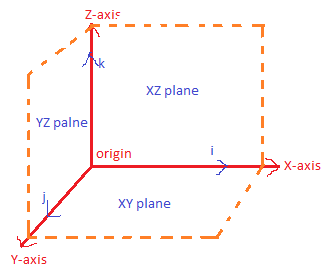
\includegraphics{x-z plane.jpeg}
    
\end{figure}  

\footnote{\url{https://www.vedantu.com/question-sets/0b332bea-6a22-4a13-971c-42e7b75218da6540201208005621542.png}}

Definiamo il piano (x-z); possiamo definire due tipi di polarizzazione: 

\begin{itemize}
    \item quando $\vec{E}$ è perpendicolare al piano (x-z), si definisce polarizzazione transversa elettrica (oppure polarizzazione TE)
    \item quando $\vec{H}$ è perpendicolare al piano (x-z), quindi $\vec{E}$ è parallelo al piano (x-z), viene definita come polarizzazione transversa magnetica (oppure polarizzazione TM)
\end{itemize}


Sia nel caso TE e TM, ricordiamo che, dato un piano di incidenza, le componenti tangenziali di $\vec{E}$ e $\vec{H}$ 
nei due piani devono essere continue. \\ 

\newpage 

\section{Onda piana TE} 

\footnote{FCE - pag 328 | 8.4.1 Polarizzazione perpendicolare \\ 
FAE - pag 354 | 8.4.1 Perpendicular Polarization} 

\begin{figure}[h]
    \centering
    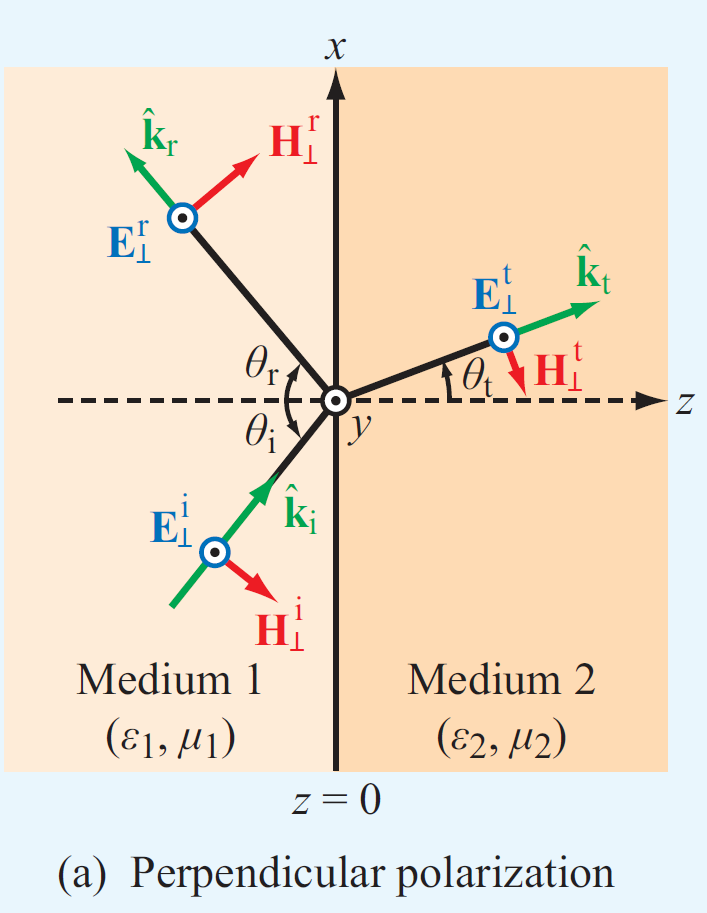
\includegraphics[scale = 0.8]{TE polarization.PNG}
    
\end{figure}    

\begin{figure}[h]
    \centering
    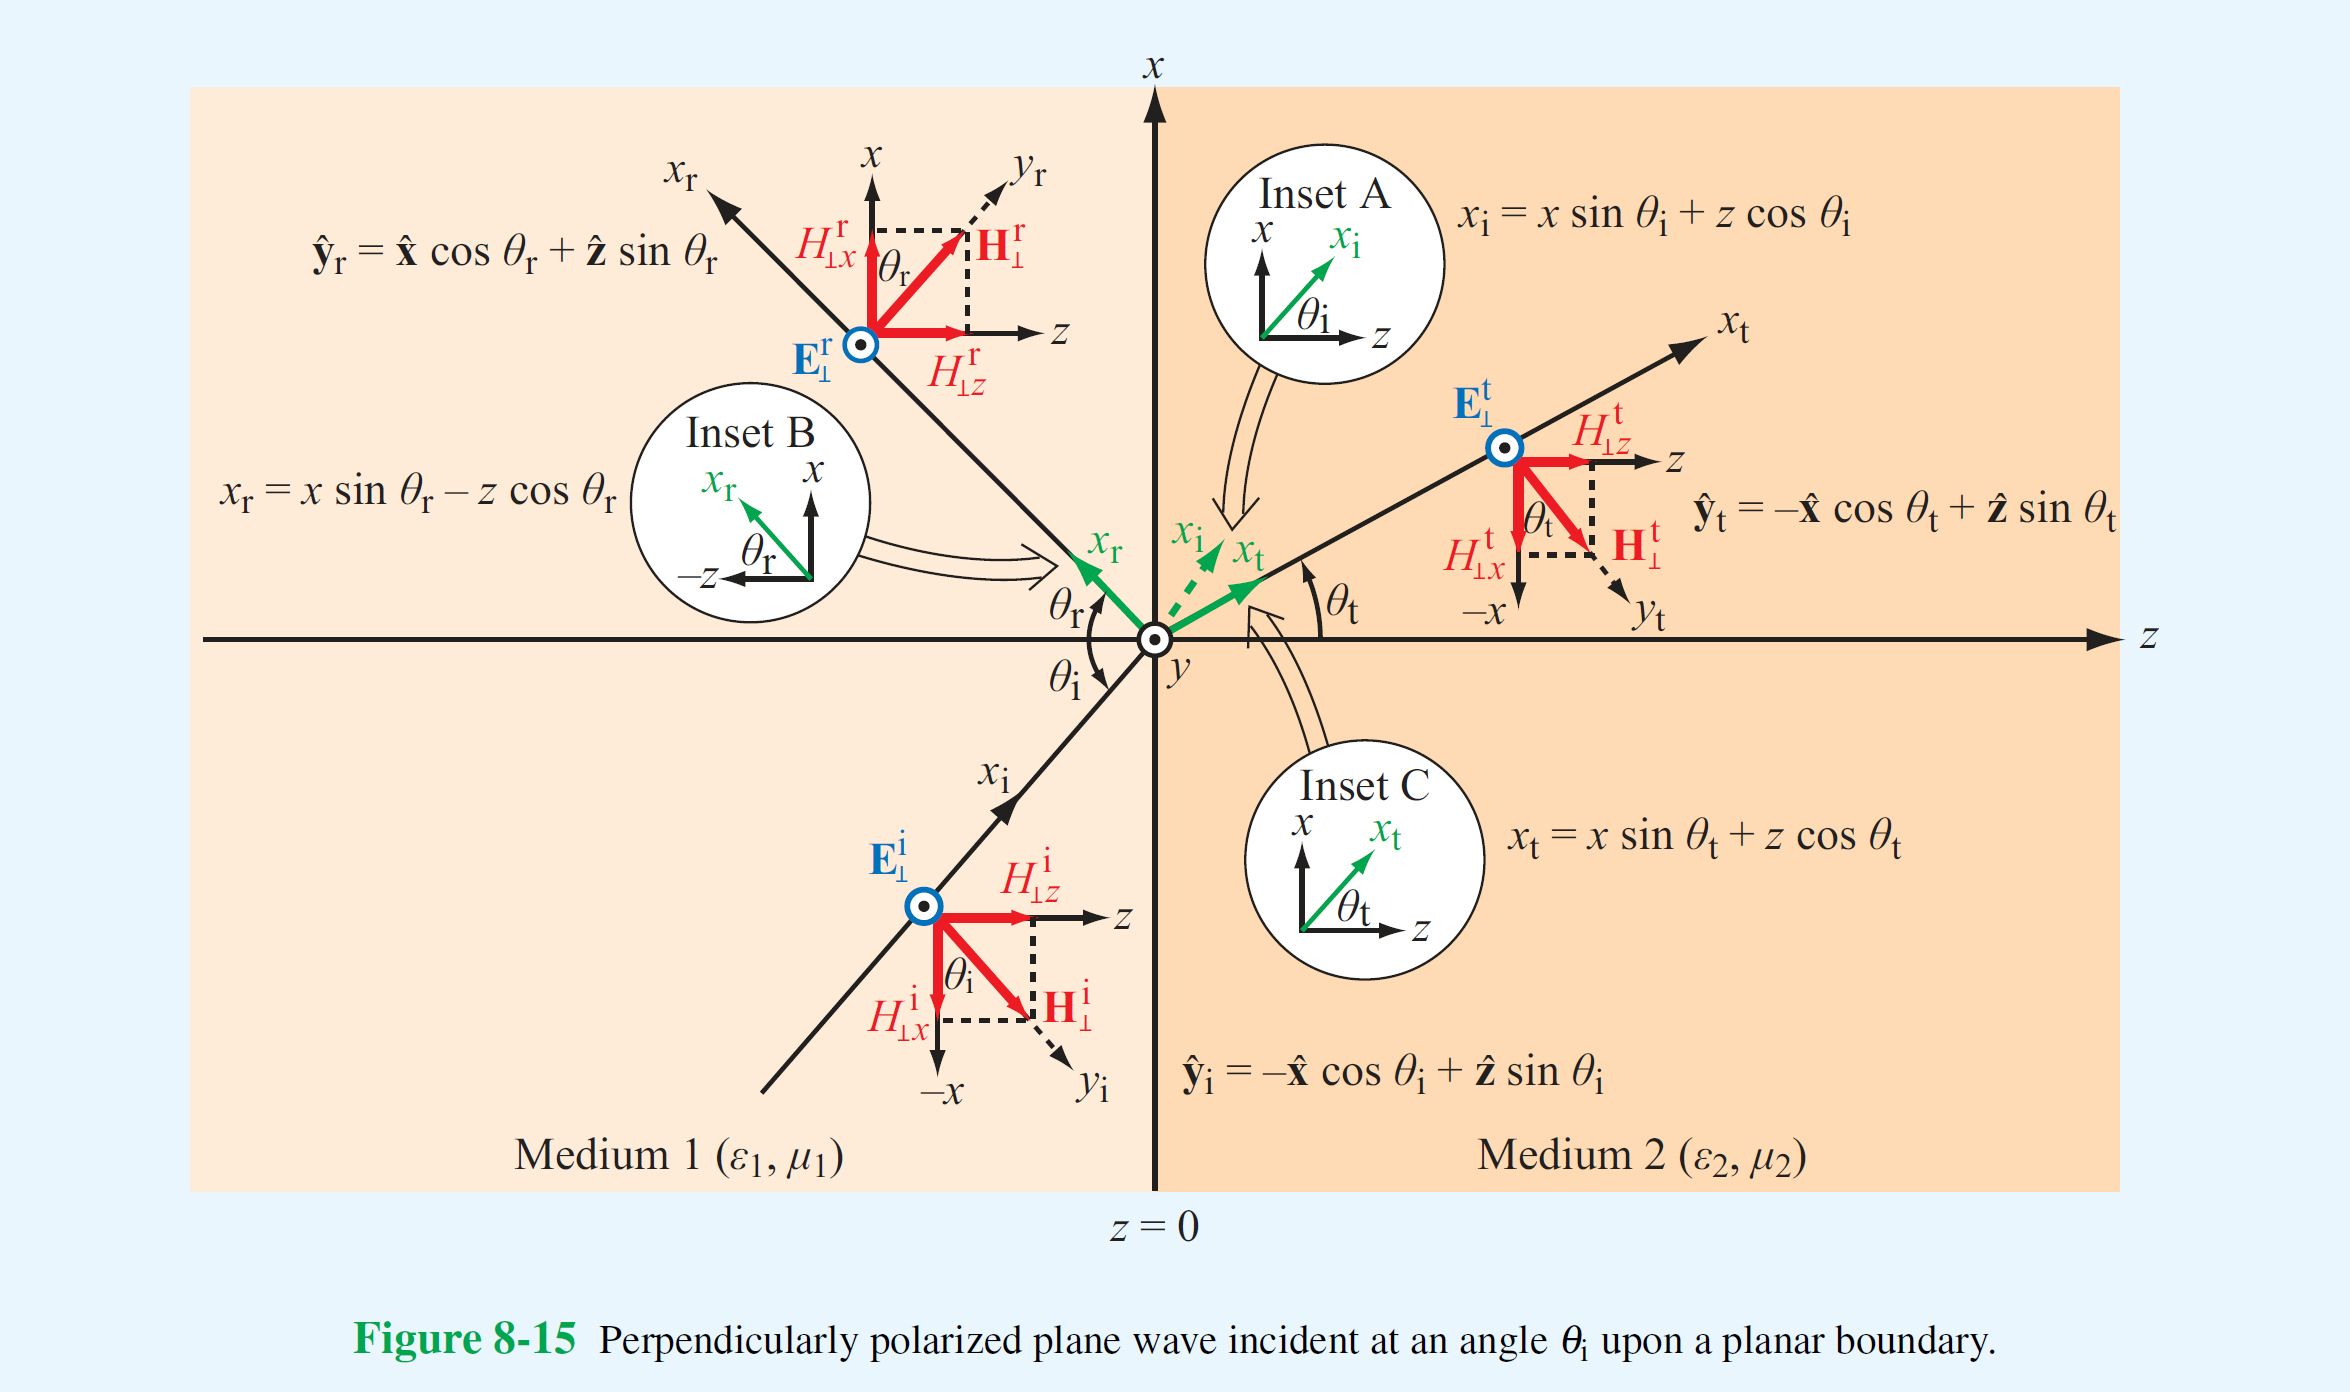
\includegraphics[scale = 0.5]{TE polarization with equations.PNG}
    
\end{figure}    

\footnote{FAE - pag 355} 

Nel mezzo 1 avremo: 

\begin{itemize}
    \item $\vec{E_\perp^{i}} $ punta in direzione $y$
    \item $\vec{H_\perp^{i}} $ punta in direzione $y_i$
\end{itemize}

Un'onda di questo tipo è descritta dalle seguenti equazioni: 

{\Large \begin{equation}
    \begin{cases}
        \vec{E_\perp^{1}} = \hat{y} E_{\perp_o}^{1} e^{-\jmath \kappa_1 x_i} \\ 
        \vec{H_\perp^{1}} = \hat{y_i} \frac{E_{\perp_o}^{1}}{\eta_1} e^{-\jmath \kappa_1 x_i}
    \end{cases}
\end{equation}}

dove: 

{\Large \begin{equation}
    \begin{cases}
        x_i = x \sin(\theta_i) + z \cos(\theta_i) \\ 
        \hat{y_i} = -\hat{x} \cos(\theta_i) + \hat{z} \sin(\theta_i)        
    \end{cases}
\end{equation}}

Scomponendo $\vec{E_\perp^{1}}$ in onda incidente e onda riflessa, avremo che: 

{\Large \begin{equation}
    \vec{E_\perp^{1}} = \vec{E_\perp^{i}} + \vec{E_\perp^{r}}
\end{equation}}

\textbf{Onda incidente:} 

{\Large \begin{equation}
    \begin{cases}
        \vec{E_\perp^{i}} = \hat{y} E_{\perp_o}^{i} e^{-\jmath \kappa_1 x_i} \\ 
        \vec{H_\perp^{i}} = \hat{y_i} \frac{E_{\perp_o}^{i}}{\eta_1} e^{-\jmath \kappa_1 x_i}
    \end{cases}
\end{equation}}

\textbf{Onda riflessa:} 

{\Large \begin{equation}
    \begin{cases}
        \vec{E_\perp^{r}} = \hat{y} E_{\perp_o}^{r} e^{-\jmath \kappa_1 x_r} \\ 
        \vec{H_\perp^{r}} = \hat{y_r} \frac{E_{\perp_o}^{r}}{\eta_1} e^{-\jmath \kappa_1 x_r}
    \end{cases}
\end{equation}}


dove: 

{\Large \begin{equation}
    \begin{cases}
        x_r = x \sin(\theta_r) - z \cos(\theta_r) \\ 
        \hat{y_r} = \hat{x} \cos(\theta_r) + \hat{z} \sin(\theta_r)        
    \end{cases}
\end{equation}}

Nel mezzo 2 avremo solo l'onda trasmessa. \\ 

\textbf{Onda trasmessa:} 

{\Large \begin{equation}
    \begin{cases}
        \vec{E_\perp^{t}} = \hat{y} E_{\perp_o}^{t} e^{-\jmath \kappa_2 x_t} \\ 
        \vec{H_\perp^{t}} = \hat{y_t} \frac{E_{\perp_o}^{t}}{\eta_2} e^{-\jmath \kappa_2 x_t}
    \end{cases}
\end{equation}}

dove: 

{\Large \begin{equation}
    \begin{cases}
        x_t = x \sin(\theta_t) + z \cos(\theta_t) \\ 
        \hat{y_t} = -\hat{x} \cos(\theta_t) + \hat{z} \sin(\theta_t)        
    \end{cases}
\end{equation}}


Dal momento che i campi elettrici nel mezzo 1 e nel mezzo 2 presentano solo componenti 
lungo $\hat{y}$, la condizione al contorno di $\vec{E}$ è: 

{\Large \begin{equation}
    (\vec{E_{\perp_y}^{i}} + \vec{E_{\perp_y}^{r}} )\big|_{z=0} = 
    \vec{E_{\perp_y}^{t}}\big|_{z=0}
\end{equation}} 

\begin{tcolorbox}
    Il simbolo matematico $\big|$ indica che l'equazone e/o la formula a sinistra del segno 
    viene calcolata, o propriamente si dice valutata, nel punto inidicato in basso a destra del segno. \\ \\
    Per esempio: \\ 

    $\vec{E_{\perp_y}^{t}}\big|_{z=0}$ \\ 

    si legge: \\ 
    la componete y del vettore del campo elettrico con polarizzazione TE trasmessa nella regione 2 
    viene valutata nel punto $z=0$ 
\end{tcolorbox}

Svolgendo diversi passaggi algebrici, avremo che: 

{\Large \begin{equation}
    E_{\perp_o}^{i} e^{-\jmath \kappa_1 x \sin(\theta_i)} + E_{\perp_o}^{r} e^{-\jmath \kappa_1 x \sin(\theta_r)} = 
    E_{\perp_o}^{t} e^{-\jmath \kappa_2 \sin(\theta_t)}
\end{equation}}

La condizione al contorno del campo elettrico (cioè il campo lungo x) è: 

{\Large \begin{equation}
    (\vec{H_{\perp_x}^{i}} + \vec{H_{\perp_x}^{r}} )\big|_{z=0} = 
    \vec{H_{\perp_x}^{t}}\big|_{z=0}
\end{equation}} 

In formule: 

{\Large \begin{equation}
    - \frac{E_{\perp_o}^{i}}{\eta_1} \cos(\theta_i) e^{-\jmath \kappa_1 \sin(\theta_i)} + \frac{E_{\perp_o}^{r}}{\eta_1} \cos(\theta_r) e^{-\jmath \kappa_1 \sin(\theta_r)} = 
    - \frac{E_{\perp_o}^{t}}{\eta_2} \cos(\theta_t) e^{-\jmath \kappa_2 \sin(\theta_t)}    
\end{equation}}


Per soddisfare le due condizioni al contorno per ogni valore di x, tutti gli argomenti degli esponenziali devono essere uguali, quindi: 

{\Large \begin{equation}
    \kappa_1 \sin(\theta_i) = \kappa_1 \sin(\theta_r) = \kappa_2 \sin(\theta_t) 
\end{equation}}

Questa triplice uguaglianza è detta condizione di phase-matching. \\ 

Sapendo che $\theta_i = \theta_r$ e applicando il phase-matching, avremo che: 

{\Large \begin{equation}
    E_{\perp_o}^{i} + E_{\perp_o}^{r} = E_{\perp_o}^{t} 
\end{equation}} 

Cioè: 

{\Large \begin{equation}
    \frac{\cos(\theta_i)}{\eta_1} (- E_{\perp_o}^{i} + E_{\perp_o}^{r}) = 
    - \frac{\cos(\theta_t)}{\eta_2} E_{\perp_o}^{t}
\end{equation}}

Da queste due equazioni, è possibile ricavare, come il caso TEM, il coefficiente di riflessione e di trasmissione. 

{\Large \begin{equation}
    \Gamma_{TE} = \frac{E_{\perp_o}^{r}}{E_{\perp_o}^{i}} = \frac{\eta_2 \cos(\theta_i) - \eta_1 \cos(\theta_t)}{\eta_2 \cos(\theta_i) + \eta_1 \cos(\theta_t)}
\end{equation}}


\begin{tcolorbox}
    Nel caso TEM: \\ \\ $\Gamma_{TEM} = \frac{\eta_2 - \eta_1}{\eta_2 + \eta_1}$
\end{tcolorbox}


{\Large \begin{equation}
    \tau_{TE} = \frac{E_{\perp_o}^{t}}{E_{\perp_o}^{i}} = \frac{2 \eta_2 \cos(\theta_i) }{\eta_2 \cos(\theta_i) + \eta_1 \cos(\theta_t)}
\end{equation}}


\begin{tcolorbox}
    Nel caso TEM: \\ \\ $\tau_{TEM} = \frac{2 \eta_2}{\eta_2 + \eta_1}$
\end{tcolorbox}

I due coefficienti sono legati da: 

{\Large \begin{equation}
    \tau_{TE} = 1 + \Gamma_{TE} 
\end{equation}}

Utilizzando i coefficienti, possiamo scrivere la continuità in $z=0$ sapendo il valore di $E_{\perp_o}^{i} = E_1$ come: 

{\Large \begin{equation}
    E_1 \cos(1 + \Gamma_{TE}) = \tau_{TE} E_1 \cos(\theta_2)
\end{equation}} 

Diventa: 

{\Large \begin{equation}
    \frac{E_1}{\eta_1} (1 + \Gamma_{TE}) = \tau_{TE} \frac{E_2}{\eta_2}
\end{equation}} 


Se il mezzo 2 è un perfetto conduttore ($\eta_2 = 0$), allora $\Gamma_{TE} = -1$ e $\tau_{TE} = 0$. \\ 

Ricordiamo che per materiali non magneitici, $\mu_1 = \mu_2 = \mu_o$, quindi si può esprimere $\Gamma_{TE}$ grazie 
a queste sostituzioni. 


\newpage 

\section{Onda piana TM}

\footnote{FCE - pag 333 | Polarizzazione parallela \\ 
FAE - pag 359 | 8.4.2 Parallel Polarization} 

\begin{figure}[h]
    \centering
    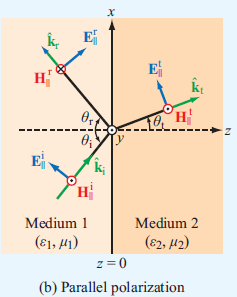
\includegraphics[scale = 0.8]{TM polarization.PNG}
    
\end{figure}   

\footnote{FAE - pag 354 } 

\begin{figure}[h]
    \centering
    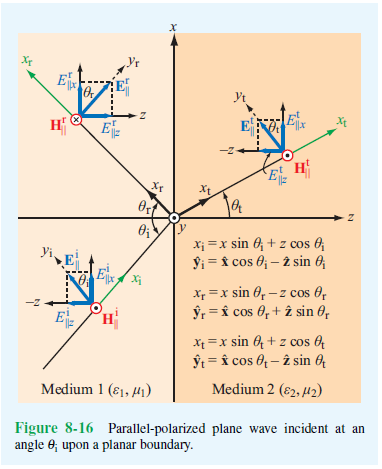
\includegraphics[scale = 0.8]{TM polarization with equations.PNG}
    
\end{figure}   

Stesso principio della polarizzazione perpendicolare TE, quindi: 

{\Large \begin{equation}
    \begin{cases}
        \vec{E_\parallel^{1}} = \vec{E_\parallel^{i}} + \vec{E_\parallel^{r}} \\ 
        \vec{H_\parallel^{1}} = \vec{H_\parallel^{i}} + \vec{H_\parallel^{r}}
    \end{cases}
\end{equation}}


\textbf{Onda incidente:} 

{\Large \begin{equation}
    \begin{cases}
        \vec{E_\parallel^{i}} = \hat{y_i} E_{\parallel_o}^{i} e^{-\jmath \kappa_1 x_i} \\ 
        \vec{H_\parallel^{i}} = \hat{y} \frac{E_{\parallel_o}^{i}}{\eta_1} e^{-\jmath \kappa_1 x_i}
    \end{cases}
\end{equation}} 

dove: 

{\Large \begin{equation}
    \begin{cases}
        x_i = x \sin(\theta_i) + z \cos(\theta_i) \\ 
        \hat{y_i} = \hat{x} \cos(\theta_i) - \hat{z} \sin(\theta_i)        
    \end{cases}
\end{equation}}

\textbf{Onda riflessa:} 

{\Large \begin{equation}
    \begin{cases}
        \vec{E_\parallel^{r}} = \hat{y_r} E_{\parallel_o}^{r} e^{-\jmath \kappa_1 x_r} \\ 
        \vec{H_\parallel^{r}} = - \hat{y} \frac{E_{\parallel_o}^{r}}{\eta_1} e^{-\jmath \kappa_1 x_r}
    \end{cases}
\end{equation}} 

dove: 

{\Large \begin{equation}
    \begin{cases}
        x_r = x \sin(\theta_r) - z \cos(\theta_r) \\ 
        \hat{y_r} = \hat{x} \cos(\theta_r) + \hat{z} \sin(\theta_r)        
    \end{cases}
\end{equation}}


\textbf{Onda trasmessa:} 

{\Large \begin{equation}
    \begin{cases}
        \vec{E_\parallel^{t}} = \hat{y_t} E_{\parallel_o}^{t} e^{-\jmath \kappa_2 x_t} \\ 
        \vec{H_\parallel^{t}} = \hat{y} \frac{E_{\parallel_o}^{t}}{\eta_2} e^{-\jmath \kappa_2 x_t}
    \end{cases}
\end{equation}} 

dove: 

{\Large \begin{equation}
    \begin{cases}
        x_t = x \sin(\theta_t) + z \cos(\theta_t) \\ 
        \hat{y_t} = \hat{x} \cos(\theta_t) - \hat{z} \sin(\theta_t)        
    \end{cases}
\end{equation}}

Facendo la stessa cosa che abbiamo fatto con la polarizzazione TE per la continuità dei 
componenti trasversali di $\vec{E}$ e $\vec{H}$ in $z=0$, possiamo ricavarci i coeffienti di Fresnel per la polarizzazione parallela. 

{\Large \begin{equation}
    \Gamma_{TM} = \frac{E_{\parallel_o}^{r}}{E_{\parallel_o}^{i}} = \frac{\eta_2 \cos(\theta_t) - \eta_1 \cos(\theta_i)}{\eta_2 \cos(\theta_t) + \eta_1 \cos(\theta_i)}
\end{equation}}

{\Large \begin{equation}
    \tau_{TM} = \frac{E_{\parallel_o}^{t}}{E_{\parallel_o}^{i}} = \frac{2 \eta_2 \cos(\theta_i) }{\eta_2 \cos(\theta_t) + \eta_1 \cos(\theta_i)}
\end{equation}} 

Si può dimostrare che: 

{\Large \begin{equation}
    \tau_{TM} = (1 + \Gamma_{TM}) \frac{\cos(\theta_i)}{\cos(\theta_t)} 
\end{equation}} 


Come il caso TE, se il mezzo 2 è un perfetto conduttore ($\eta_2 = 0$), allora $\Gamma_{TM} = -1$ e $\tau_{TM} = 0$. \\ 

Ricordiamo che per materiali non magneitici, $\mu_1 = \mu_2 = \mu_o$, quindi si può esprimere $\Gamma_{TM}$ grazie 
a queste sostituzioni. 


\newpage 

\section{Angolo di Brewster} 

\footnote{FCE - pag 335 | 8.4.3 Angolo di Brewster \\ 
FAE - pag 360 | 8.4.3 Brewster angle } 

L'angolo di Brewster $\theta_B$ è definito come l'angolo di incidenza $\theta_i$ per il quale $\Gamma = 0$. \\ 

Dalla definizione di $\Gamma_{TE}$: 

{\Large \begin{equation}
    \Gamma_{TE} = \frac{E_{\perp_o}^{r}}{E_{\perp_o}^{i}} = \frac{\eta_2 \cos(\theta_i) - \eta_1 \cos(\theta_t)}{\eta_2 \cos(\theta_i) + \eta_1 \cos(\theta_t)}
\end{equation}}

{\Large \begin{equation}
    \Gamma_{TE} = 0 \iff \eta_2 \cos(\theta_i) - \eta_1 \cos(\theta_t) = 0 
    \iff \eta_2 \cos(\theta_i) = \eta_1 \cos(\theta_t)
\end{equation}} 


\begin{tcolorbox}
    $\iff$ è il simbolo matematico per dire "se e solo se"
\end{tcolorbox}

Facendo le dovute sostituzioni (omesse per semplicità) a $\Gamma_{TE}$ avremo che: 

{\Large \begin{equation}
    \sin(\theta_{B_{TE}}) = \sqrt{\frac{1 - \frac{\mu_1 \varepsilon_2}{\mu_2 \varepsilon_1}}{1 - (\frac{\mu_1}{\mu_2} )^{2}}}
\end{equation}} 

Per materiali non magneitici, $\mu_1 = \mu_2 $ quindi il denominatore della divisione è $=0$, 
quindi $\theta_{B_{TE}}$ non esiste. \\ \\ 

Per le onde TM, si fa lo stesso procedimento e avremo che: 

{\Large \begin{equation}
    \sin(\theta_{B_{TM}}) = \sqrt{\frac{1 - \frac{\mu_2 \varepsilon_1}{\mu_1 \varepsilon_2}}{1 - (\frac{\varepsilon_1}{\varepsilon_2} )^{2}}}
\end{equation}} 

Per materiali non magneitici, $\mu_1 = \mu_2$ quindi: 

{\Large \begin{equation}
    \begin{split}
        \theta_{B_{TM}} 
        &= \arcsin(\sqrt{\frac{1}{1 + \frac{\varepsilon_1}{\varepsilon_2}}}) 
        \\
        &= \arctan (\sqrt{\frac{\varepsilon_2}{\varepsilon_1}}) 
    \end{split}
\end{equation}}

\begin{tcolorbox}
    $\arcsin = \sin ^{-1}$ cioè l'inverso della funzione $\sin$
\end{tcolorbox}



\footnote{Slide prof | Incidenza obliqua su un piano di massa | Pag 20}

L'angolo di Brewster viene definito anche come angolo polizzatore perchè se un'onda non polarizzata (quindi 
contiene sia un'onda TE che TM) è incidente a $\theta_{B_{TM}}$, allora la componente TM passa nel mezzo 2, 
mentre la componente TE viene riflessa e polarizzata. 


\begin{figure}[h]
    \centering
    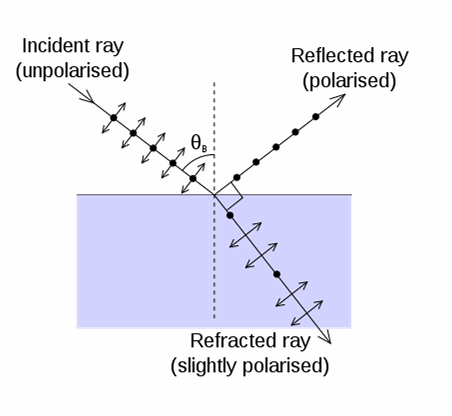
\includegraphics[scale = 0.3]{Angolo polarizzatore.PNG}
    
\end{figure}  

\newpage

\section{Vettore di Poynting per onde TE e TM} 

\footnote{FCE - pag 337 | 8.5 Riflettività e trasmissitività \\ 
FAE - pag 361 | 8.5 Reflectivity and Trasmissitivity}

\begin{figure}[h]
    \centering
    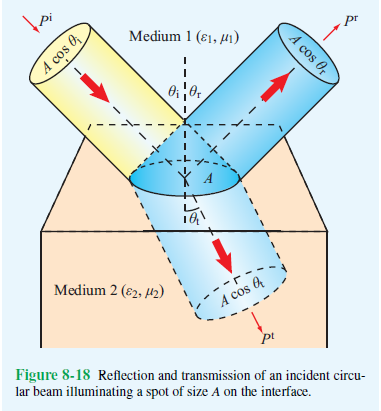
\includegraphics[scale = 0.8]{Vettore Poynting TE e TM.PNG}
    
\end{figure}  

Consideriamo le onde con polarizzazione TE. \\ 

La densità di potenza dei fasci incidente, riflesso e trasmesso sono: 

{\Large \begin{equation}
    \begin{cases}
        S_\perp ^{i} = \frac{\left|E_{\perp_o} ^{i}\right| ^{2}}{2 \eta_1} \\ 
        S_\perp ^{r} = \frac{\left|E_{\perp_o} ^{r}\right| ^{2}}{2 \eta_1} \\ 
        S_\perp ^{t} = \frac{\left|E_{\perp_o} ^{t}\right| ^{2}}{2 \eta_2}
    \end{cases}
\end{equation}}


Consideriamo A come la regione illuminata dalle onde, avremo: 

{\Large \begin{equation}
    \begin{cases}
        A_i = A \cos(\theta_i) \\ 
        A_r = A \cos(\theta_r) \\ 
        A_t = A \cos(\theta_t)  
    \end{cases}
\end{equation}}

Le potenze medie trasportate dalle onde saranno: 

{\Large \begin{equation}
    \begin{cases}
        P_{TE} ^{i} = S_\perp ^{i} A_i = \frac{\left|E_{\perp_o} ^{i}\right| ^{2}}{2 \eta_1} A \cos(\theta_i) \\ 
        P_{TE} ^{r} = S_\perp ^{r} A_r = \frac{\left|E_{\perp_o} ^{i}\right| ^{2}}{2 \eta_1} A \cos(\theta_r) \\ 
        P_{TE} ^{t} = S_\perp ^{t} A_t = \frac{\left|E_{\perp_o} ^{t}\right| ^{2}}{2 \eta_2} A \cos(\theta_t) 
    \end{cases}
\end{equation}}

Definiamo R come indice di riflettanza: 

{\Large \begin{equation}
    R_{TE} = \frac{P_{TE} ^{r}}{P_{TE} ^{i}} = \frac{\left|E_{\perp_o} ^{r}\right| ^{2} \cos(\theta_r)}{\left|E_{\perp_o} ^{i}\right| ^{2} \cos(\theta_i)} = \left|\frac{E_{\perp_o} ^{r}}{E_{\perp_o} ^{i}}\right| ^{2} = \left|\Gamma_\perp\right|\ ^{2}  
\end{equation}}

in cui $\theta_r = \theta_i$. \\ 

Indichiamo con T la trasmittanza: 

{\Large \begin{equation}
    T_{TE} = \frac{P_\perp ^{t}}{P_\perp ^{i}} = \frac{\left|E_{\perp_o} ^{t}\right| ^{2}}{\left|E_{\perp_o} ^{i}\right| ^{2}} \frac{\eta_1}{\eta_2} \frac{A \cos(\theta_t)}{A \cos(\theta_i)} = 
    \left|\tau_{TE}\right| ^{2} (\frac{\eta_1 \cos(\theta_t)}{\eta_2 \cos(\theta_i)})
\end{equation}}

Come il caso TE, possiamo esprimere la riflettanza e la trasmittanza nel caso TM: 

{\Large \begin{equation}
    \begin{cases}
        R_{TM} = \frac{P_{TM} ^{r}}{P_{TM} ^{i}} = \left|\Gamma_{TM}\right| ^{2} \\ 
        T_{TM} = \frac{P_{TM} ^{t}}{P_{TM} ^{i}} = \left|\tau_{TM}\right| ^{2}  (\frac{\eta_1 \cos(\theta_t)}{\eta_2 \cos(\theta_i)})
    \end{cases}    
\end{equation}}

Possiamo dire che, per la converzione dell'energia. che: 

{\Large \begin{equation}
    P_{TE} ^{i} = P_{TE} ^{r} + P_{TE} ^{t} 
\end{equation}} 

cioè: 

{\Large \begin{equation}
    \begin{cases}
        R_\perp + T_\perp = 1 \\ 
        R_\parallel + T_\parallel = 1 
    \end{cases}
\end{equation}} 


Per $\theta_B$, $R_{TM} = 0$ e $\tau_{TM} = 1$. \\ \\ 

Per riassumere: 

\begin{figure}[h]
    \centering
    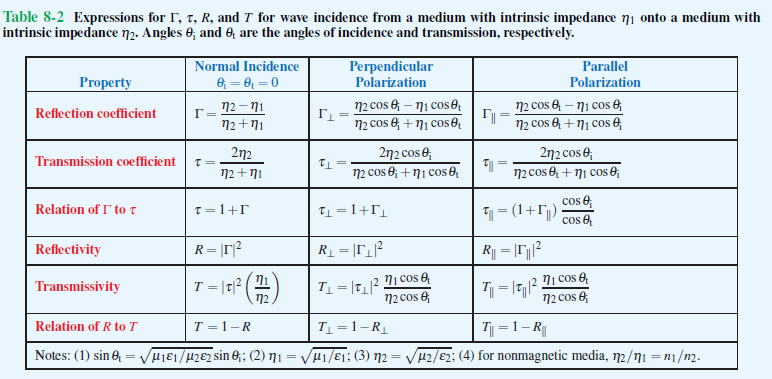
\includegraphics[scale = 0.8]{Tabella coefficienti onde piane.PNG}
    
\end{figure}  

\footnote{FAE - pag 363} 

\newpage 


